% !TeX root = surprises.tex

\chapter{Teoría de Ramsey}\label{c.ramsey}

%%%%%%%%%%%%%%%%%%%%%%%%%%%%%%%%%%%%%%%%%%%%%%%%%%%%%%%%%%%

La teoría de Ramsey es una rama de la combinatoria que plantea preguntas del tipo ¿Qué tamaño debe tener un conjunto para que, si se divide en subconjuntos, al menos uno de ellos tenga una determinada propiedad?
Los resultados de la teoría de Ramsey son difíciles de demostrar y quedan muchos problemas abiertos. En este capítulo presentamos casos sencillos de cuatro problemas para dar una idea de este fascinante tema: Ternaewde Schur (Sec.~\ref{s.schur})---ternas de enteros tales que $a+b=c$, ternas pitagóricas (Sec.~\ref{s.pyth})---ternas de enteros tales que $a^2+b^2=c^2$, el problema de van der Waarden (Sec.~\ref{s.van}) que se refiere a secuencias de números, y el teorema de Ramsey (Sec.~\ref{s.ramsey}) sobre grafos coloreados. La sección~\ref{s.bounds} muestra cómo se puede utilizar el método probabilístico en combinatoria para desarrollar una cota inferior para los números de Ramsey.

El problema de las ternas pitagóricas se ha resuelto recientemente con ayuda de ordenadores, utilizando un método relativamente nuevo llamado resolución SAT. Para los lectores familiarizados con la lógica proposicional, la sección~\ref{s.sat} ofrece una visión general de cómo se hace.

La sección~\ref{s.plimpton} describe las ternas pitagóricas tal y como las conocían los babilonios hace cuatro mil años.

Terminología: \emph{Monocromático} significa del mismo color.

%%%%%%%%%%%%%%%%%%%%%%%%%%%%%%%%%%%%%%%%%%%%%%%%%%%%%%%%%%%

\section{Ternas de Schur}\label{s.schur}

\begin{definition}
Dada \emph{any} descomposición del conjunto de enteros positivos:
\[
S(n)=\{1,\ldots,n\}
\]
en dos subconjuntos disjuntos $S_1,S_2$, ¿existen $\{a,b,c\}\subseteq S_1$ o $\{a,b,c\}\subseteq S_2$ (o en ambos) tales que $a\!<\!b\!<\!c$ y $a+b=c$? Si es así, el conjunto $ {a,b,c}$ se llama terna de Schur.
\end{definition}

\begin{example} Para $n=8$, en la descomposición:
\begin{align}
S_1 = \{1,2,3,4\},\; S_2 = \{5,6,7,8\}\,,
\label{eq.schur0}
\end{align}
el conjunto $S_1$ incluye la terna de Schur $\{1,2,3\}$.
Sin embargo, la descomposición:
\begin{align}
S'_1 = \{1,2,4,8\},\; S'_2 = \{3,5,6,7\}\,,
\label{eq:schur1}
\end{align}
no contiene ningúna terna de Schur, como se puede comprobar enumerando todos las ternas de cada subconjunto.
\end{example}

\begin{theorem}
En \emph{todas} descomposiciones de $S(9)=\{1,\ldots,9\}$ en dos subconjuntos disjuntos, al menos un subconjunto contiene una terna de Schur.
\end{theorem}
Por supuesto, podríamos comprobar las $2^9=512$ descomposiciones de $S(9)$ en dos subconjuntos disjuntos, pero vamos a tratar de llegar a una demostración más sucinta.
\begin{proof}
Intentamos construir una descomposición que no contenga una terna de Schur y demostramos que las restricciones del problema lo hacen imposible. Se empieza colocando $1$ y $3$ en el subconjunto $S_1$. El $2$ debe colocarse en $S_2$ porque $1+2=3$ y estamos intentando construir una descomposición que no contenga una terna de Schur. Análogamente, el $4$ debe colocarse en $S_2$ porque $1+3=4$. Continuando, el $6$ se coloca en $S_1$ porque $2+4=6$ y el $7$ se coloca en $S_2$ porque $1+6=7$. Sin embargo, $3+6=9$ y $2+7=9$, por lo que el $9$ debe aparecer tanto en $S_1$ como en $S_2$, una contradicción. La secuencia de inferencias se muestra en la siguiente tabla:
\[
\begin{array}{l@{\hspace{2em}}l}
S_1&S_2\\\hline
1,3 & \\
1,3 & 2\\
1,3 & 2,4\\
1,3,6 & 2,4\\
1,3,6 & 2,4,7\\
1,3,6,9 & 2,4,7\\
1,3,6,9 & 2,4,7,9
\end{array}
\]
Retrocediendo, buscamos una descomposición en la que $1,3$ estén en subconjuntos distintos. Si colocamos el $5$ en $S_2$, una secuencia de inferencias conduce de nuevo a una contradicción porque el $9$ debe aparecer en ambos subconjuntos. El lector debe justificar cada una de las inferencias que se muestran en la siguiente tabla:
\[
\begin{array}{l@{\hspace{2em}}l}
S_1&S_2\\\hline
1&3\\
1 & 3,5\\
1,2&3,5\\
1,2,8&3,5\\
1,2,8&3,5,7\\
1,2,8&3,5,7,9\\
1,2,8&3,5,6,7,9\\
1,2,8,9&3,5,6,7,9
\end{array}
\]
Retrocediendo de nuevo, tratamos de colocar el $5$ en $S_1$, pero eso también conduce a una contradicción, como se muestra en la siguiente tabla:
\[
\begin{array}{l@{\hspace{2em}}l}
S_1&S_2\\\hline
1&3\\
1,5& 3\\
1,5&3,4\\
1,5&3,4,6\\
1,2,5&3,4,6\\
1,2,5&3,4,6,7\\
1,2,5,7&3,4,6,7
\end{array}
\]
De ello se deduce que no existe ninguna descomposición que no incluya una terna de Schur.
\end{proof}
Issai Schur demostró el siguiente teorema:
\begin{theorem}[Schur]
Para cada $k\geq 2$ existe un $n$ mínimo tal que en cualquier descomposición disjunta de $S(n)$ en $k$ subconjuntos, al menos uno de los subconjuntos debe contener una terna de Schur.
\end{theorem}

%%%%%%%%%%%%%%%%%%%%%%%%%%%%%%%%%%%%%%%%%%%%%%%%%%%%%%%%%%%

\section{Ternas pitagóricas}\label{s.pyth}

\begin{definition}
Dada \emph{una} descomposición cualquiera del conjunto de enteros positivos:
\[
S(n)=\{1,\ldots,n\}
\]
en dos subconjuntos disjuntos $S_1,S_2$, ¿existen $\{a,b,c\}\subseteq S_1$ o $\{a,b,c\}\subseteq S_2$ (o en ambos) tal que $a\!<\!b\!<\!c$ y $a^2+b^2=c^2$? Si es así, $ {a,b,c}$ se llama \emph{ternas pitagórica}.\index{Pythagorean triples}
\end{definition}

\begin{example}
Para $n=10$, en la descomposición en números pares e impares:
\[
S_1 = \{1,3,5,7,9\},\; S_2=\{2,4,6,8,10\}\,,
\]
no hay ternas pitagóricas en $S_1$ pero $\{6,8,10\}$ en $S_2$ es una terna pitagórica ya que $6^2+8^2=10^2$.
\end{example}

Marijn J.H. Heule y Oliver Kullmann demostraron los siguientes teoremas. Su método de demostración se discute en la sección ~\ref{s.sat}.

\begin{theorem}
Para todo $n\leq 7824$, existe \emph{alguna} descomposición de $S(n)$ en dos subconjuntos disjuntos tal que ambos subconjuntos \emph{no contienen} una terna pitagórica.
\end{theorem}

\begin{theorem}
Para todo $n\geq 7825$, en \emph{todas} las descomposiciones de $S(n)$ en dos subconjuntos disjuntos al menos un subconjunto \emph{contiene} una terna pitagórica.
\end{theorem}
Es imposible comprobar todas las descomposiciones $2^{7825}$ de $S(7825)$. Si pudiéramos comprobar una descomposición cada microsegundo, $2^{7825}$; \textrm{microsegundos}$\;\approx 10^{600}\; \textrm{años}$, mientras que la edad estimada del universo es sólo de unos $10^{10}$ años.

%%%%%%%%%%%%%%%%%%%%%%%%%%%%%%%%%%%%%%%%%%%%%%%%%%%%%%%%%%%

\section{El problema de Van der Waerden}\label{s.van}

Consideremos las secuencias de ocho puntos de colores en la figura~\ref{f.vdw1}. En la secuencia superior hay puntos rojos en las posiciones $(1,2,3)$ y puntos azules en las posiciones $(4,5,6)$. En cada caso, las posiciones forman una progresión aritmética. Del mismo modo, en la secuencia del medio, los puntos rojos en las posiciones $(1,3,5)$ forman una progresión aritmética. Sin embargo, en la secuencia inferior no hay ningún conjunto de tres puntos monocromáticos cuyas posiciones formen una progresión aritmética. 
Las ternas de puntos rojos están en las posiciones $(1,2,5)$, $(1,2,6)$, $(2,5,6)$, ninguna de las cuales forma progresiones aritméticas, y lo mismo para los puntos azules.

\begin{figure}[htb]
\begin{center}
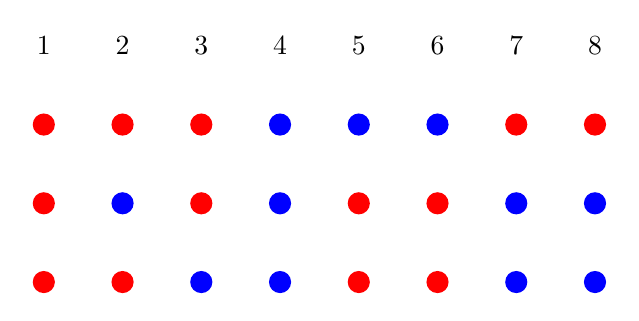
\begin{tikzpicture}
\foreach \x in {1,2,3,4,5,6,7,8} {
  \node at (\x,3) {$\x$};
}
\foreach \x/\col in {1/red,2/red,3/red,4/blue,5/blue,6/blue,7/red,8/red} {
  \fill[\col] (\x,2) circle(4pt);
}
\foreach \x/\col in {1/red,2/blue,3/red,4/blue,5/red,6/red,7/blue,8/blue} {
  \fill[\col] (\x,1) circle(4pt);
}
\foreach \x/\col in {1/red,2/red,3/blue,4/blue,5/red,6/red,7/blue,8/blue} {
  \fill[\col] (\x,0) circle(4pt);
}
\end{tikzpicture}
\end{center}
\caption{Problema de van der Waerden para ocho puntos de color}\label{f.vdw1}
\end{figure}

Con nueve puntos \emph{cualquier} coloración \emph{debe} contener una secuencia de tres puntos monocromáticos que formen una progresión aritmética. Por ejemplo, añadamos un punto rojo o un punto azul al final de la secuencia inferior de la figura~\ref{f.vdw1} para obtener las secuencias de la figura~\ref{f.vdw2}. En la secuencia superior hay puntos rojos en las posiciones $(1,5,9)$, una progresión aritmética, y en la secuencia inferior hay puntos azules en las posiciones $(7,8,9)$, también una progresión aritmética.
\begin{figure}[htb]
\begin{center}
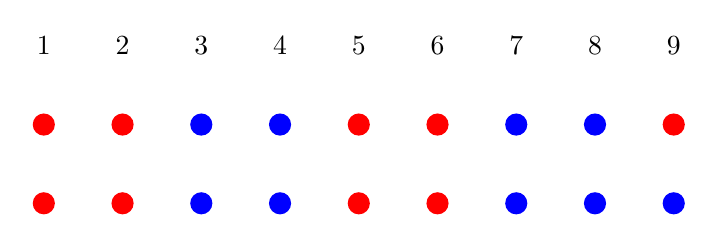
\begin{tikzpicture}
\foreach \x in {1,2,3,4,5,6,7,8,9} {
  \node at (\x,2) {$\x$};
}
\foreach \x/\col in {1/red,2/red,3/blue,4/blue,5/red,6/red,7/blue,8/blue,9/red} {
  \fill[\col] (\x,1) circle(4pt);
}
\foreach \x/\col in {1/red,2/red,3/blue,4/blue,5/red,6/red,7/blue,8/blue,9/blue} {
  \fill[\col] (\x,0) circle(4pt);
}
\end{tikzpicture}
\end{center}
\caption{Problema de van der Waerden para nueve puntos de color}\label{f.vdw2}
\end{figure}

Bartel L. van der Waerden planteó el siguiente problema: Para cualquier número entero positivo $k$, ¿cuál es el menor número $n$ tal que \emph{cualquier} secuencia de $n$ puntos coloreados \emph{debe} contener una secuencia de $k$ puntos monocromáticos que formen una progresión aritmética? Para $k=3$, $n=9$, como se ha demostrado anteriormente para una descomposición. El siguiente resultado es más difícil de demostrar: para $k=4$, $n=35$.

%%%%%%%%%%%%%%%%%%%%%%%%%%%%%%%%%%%%%%%%%%%%%%%%%%%%%%%%%%%

\section{Teorema de Ramsey}\label{s.ramsey}

Colorear las aristas de $K_5$, el grafo completo en $5$ vértices, con dos colores como se muestra en la figura~\ref{f.ramsey5}. No hay subgrafos monocromáticos $K_3$ (triángulos) en el grafo. La figura~\ref{f.ramsey6} muestra una coloración de $K_6$ y es fácil ver que hay triángulos monocromáticos $\triangle ACE$ y $\triangle BDF$. En esta sección demostramos un caso sencillo de un teorema de Frank P. Ramsey sobre la existencia de subconjuntos con cierta propiedad.
\begin{figure}[ht]
\begin{minipage}{.45\textwidth}
\begin{center}
\begin{tikzpicture}
\node (pentagon) [minimum size=5cm,regular polygon,regular polygon sides=5] at (0,0) {};
\draw[red]  (pentagon.corner 1) node[black,above] {$A$} -- (pentagon.corner 2);
\draw[red]  (pentagon.corner 2) node[black,left] {$B$} -- (pentagon.corner 3);
\draw[red]  (pentagon.corner 3) node[black,left] {$C$} -- (pentagon.corner 4);
\draw[red]  (pentagon.corner 4) node[black,right] {$D$} -- (pentagon.corner 5);
\draw[red]  (pentagon.corner 5) node[black,right] {$E$} -- (pentagon.corner 1);
\draw[dashed,blue] (pentagon.corner 1) -- (pentagon.corner 3);
\draw[dashed,blue] (pentagon.corner 1) -- (pentagon.corner 4);
\draw[dashed,blue] (pentagon.corner 2) -- (pentagon.corner 4);
\draw[dashed,blue] (pentagon.corner 2) -- (pentagon.corner 5);
\draw[dashed,blue] (pentagon.corner 3) -- (pentagon.corner 5);
\end{tikzpicture}
\caption{Una coloración de $K_5$ con dos colores}\label{f.ramsey5}
\end{center}
\end{minipage}
\hfill
\begin{minipage}{.45\textwidth}
\begin{center}
\begin{tikzpicture}
\node (hexagon) [minimum size=5cm,regular polygon,regular polygon sides=6] at (0,0) {};
\draw[red]  (hexagon.corner 1) node[black,above] {$A$} -- (hexagon.corner 2);
\draw[red]  (hexagon.corner 2) node[black,above] {$B$} -- (hexagon.corner 3);
\draw[red]  (hexagon.corner 3) node[black,left] {$C$} -- (hexagon.corner 4);
\draw[red]  (hexagon.corner 4) node[black,left] {$D$} -- (hexagon.corner 5);
\draw[red]  (hexagon.corner 5) node[black,right] {$E$} -- (hexagon.corner 6);
\draw[red]  (hexagon.corner 6) node[black,right] {$F$} -- (hexagon.corner 1);
\draw[dashed,blue] (hexagon.corner 1) -- (hexagon.corner 3);
\draw[dashed,blue] (hexagon.corner 1) -- (hexagon.corner 4);
\draw[dashed,blue] (hexagon.corner 1) -- (hexagon.corner 5);
\draw[dashed,blue] (hexagon.corner 2) -- (hexagon.corner 4);
\draw[dashed,blue] (hexagon.corner 2) -- (hexagon.corner 5);
\draw[dashed,blue] (hexagon.corner 2) -- (hexagon.corner 6);
\draw[dashed,blue] (hexagon.corner 3) -- (hexagon.corner 5);
\draw[dashed,blue] (hexagon.corner 3) -- (hexagon.corner 6);
\draw[dashed,blue] (hexagon.corner 4) -- (hexagon.corner 6);
\end{tikzpicture}
\caption{Una coloración de $K_6$ con dos colores}\label{f.ramsey6}
\end{center}
\end{minipage}
\end{figure}

\begin{definition}
$R(k)$, el número de Ramsey para $k$, es el menor número $n$ tal que en cualquier coloración de $K_{n}$, el grafo completo de $n$ vértices, con dos colores hay un subgrafo monocromático completo $K_k$.
\end{definition}
\index{Ramsey's theorem}
\begin{theorem}[Ramsey]
$\quad R(3)=6$.\label{thm.ramsey}
\end{theorem}

\begin{proof}\index{Ramsey's theorem!proof that $R(3)=6$}
La figura~\ref{f.ramsey5} muestra que $R(3)>5$. Para demostrar que $R(3)\leq 6$, considere cualquier vértice $v$ en $K_6$. $v$ está conectado con otros cinco vértices, y cuando las aristas se colorean con dos colores debe haber al menos tres aristas monocromáticas incidentes con $v$. 

En la figura~\ref{f.ramsey4a}, $\overline{AB}, \overline{AC}, \overline{AE}$ están coloreadas de rojo. Dado que el grafo es completo todos los vértices están conectados, por lo que si cualquiera de las aristas $\overline{BC}$, $\overline{BE}$, $\overline{CE}$ es de color rojo, digamos $\overline{BE}$, se forma un triángulo rojo $\triangle ABE$. De lo contrario, las tres aristas de estos bordes son de color azul y forman un triángulo azul (Fig.~\ref{f.ramsey4b}).
\end{proof}

El teorema se puede generalizar a cualquier número de colores, así como a coloraciones en las que los tamaños de los subgrafos no son iguales. $R(r,b,g)$ es el grafo completo más pequeño tal que en cualquier coloración con tres colores debe haber subgrafos completos con $r$ aristas rojas, $b$ aristas azules y $g$ aristas verdes.

\begin{figure}[t]
\begin{minipage}{.45\textwidth}
\begin{center}
\begin{tikzpicture}
\node (hexagon) [minimum size=5cm,regular polygon,regular polygon sides=6] at (0,0) {};
\draw[red]  (hexagon.corner 1) node[black,above] {$A$} -- (hexagon.corner 2) node[black,above] {$B$};
\draw[blue,dashed]  (hexagon.corner 1) -- (hexagon.corner 6) node[black,right] {$F$};
\draw[red] (hexagon.corner 1) -- (hexagon.corner 3) node[black,below] {$C$};
\draw[blue,dashed] (hexagon.corner 1) -- (hexagon.corner 4) node[black,right] {$D$};
\draw[red] (hexagon.corner 1) -- (hexagon.corner 5) node[black,right] {$E$};
\end{tikzpicture}
\caption{Un vértice de $K_6$}\label{f.ramsey4a}
\end{center}
\end{minipage}
\hfill
\begin{minipage}{.45\textwidth}
\begin{center}
\begin{tikzpicture}
\node (hexagon) [minimum size=5cm,regular polygon,regular polygon sides=6] at (0,0) {};
\draw[very thick,red]  (hexagon.corner 1) node[black,above] {$A$} -- (hexagon.corner 2) node[black,above] {$B$};
\draw[blue,dashed]  (hexagon.corner 1) -- (hexagon.corner 6) node[black,right] {$F$};
\draw[red] (hexagon.corner 1) -- (hexagon.corner 3) node[black,below] {$C$};
\draw[blue,dashed] (hexagon.corner 1) -- (hexagon.corner 4) node[black,right] {$D$};
\draw[very thick,red] (hexagon.corner 1) -- (hexagon.corner 5) node[black,right] {$E$};
\draw[very thick,red] (hexagon.corner 2) -- (hexagon.corner 5);
\draw[very thick,blue,dashed] (hexagon.corner 2) -- (hexagon.corner 3);
\draw[very thick,blue,dashed] ($(hexagon.corner 2)+(-2pt,0)$) -- ($(hexagon.corner 5)+(-2pt,0)$);
\draw[very thick,blue,dashed] (hexagon.corner 5) -- (hexagon.corner 3);
\end{tikzpicture}
\caption{Triángulos monocromáticos en $K_6$}\label{f.ramsey4b}
\end{center}
\end{minipage}
\end{figure}

%%%%%%%%%%%%%%%%%%%%%%%%%%%%%%%%%%%%%%%%%%%%%%%%%%%%%%%%%%%

\section{El método probabilístico}\label{s.bounds}

Los únicos números de Ramsey no triviales conocidos son $R(3)=6$ y $R(4)=18$. En 1947, Paul Erd\H{o}s desarrolló el \emph{método probabilístico} y lo utilizó para mostrar los límites inferior y superior de $R(k)$. Las investigaciones posteriores han mejorado ambos límites, pero sigue siendo un área de investigación importante, ya que los límites no son estrictos. Por ejemplo, se ha demostrado que $43\leq R(5) \leq 48$ y $798\leq R(10)\leq 23556$. En esta sección se utiliza la probabilidad elemental para obtener una cota inferior de $R(k)$.

Para demostrar que existe un elemento de un conjunto $S$ que tiene la propiedad $A$, demostraramos que la probabilidad de que un elemento \emph{aleatorio} de $S$ tenga la propiedad $A$ es mayor que cero. Es importante entender que el método es \emph{no constructivo}: sólo se demuestra que existe tal elemento pero no lo construye. Aunque por el Teorema~\ref{thm.ramsey} sabemos que $R(3)=6$, utilicemos el método probabilístico para obtener una cota inferior para $R(3)$.\index{Ramsey's theorem!lower bound for}
\begin{theorem}[Erd\H{o}s]
$\quad R(3) > 4$.
\end{theorem}
\begin{proof}
Dada una coloración \emph{aleatoria} de $K_n$ con dos colores, rojo y azul, consideremos un subgrafo arbitrario $K_3$, es decir, un triángulo arbitrario con $\binom{3}{2}=3$ lados. La probabilidad de que todos los lados sean de color rojo es $2^{-3}$, al igual que la probabilidad de que todos los lados sean de color azul, por lo que la probabilidad de que el triángulo sea monocromático es $2^{-3}+2^{-3}=2^{-2}=1/4$. El número de triángulos en $K_n$ es $\binom{n}{3}$, por lo que $P(n,3)$, la probabilidad de que $\emph{algún}$ triángulo contenido en una coloración aleatoria de $K_n$ sea monocromático, es:
\[
P(n,3)=\binom{n}{3}\cdot \frac{1}{4}\,.
\]
Si $P(n,3)<1$ entonces su complemento $\overline{P}(n,3)=1-P>0$, es decir, la probabilidad de que una coloración aleatoria de $K_n$ \emph{no} contenga un triángulo monocromático es mayor que cero, por lo que debe existir al menos uno.

La siguiente tabla muestra $\overline{P}(n,3)$ para varios valores de $n$, y si el valor de $\overline{P}(n,3)$ demuestra que existe una coloración sin ningún triángulo monocromático:
\[
\renewcommand*{\arraystretch}{1.1}
\begin{array}{r@{\hspace{5mm}}r@{\hspace{5mm}}r}
\hline
\noalign{\smallskip}
n & \overline{P}(n,3) & \textit{Exists}\\
\noalign{\smallskip}\hline\noalign{\smallskip}
3 & 3/4 & \textit{yes} \\
4 & 5/6 & \textit{yes}\\
5 & -3/7 & \textrm{--}\\
\noalign{\smallskip}
 \hline
 \end{array}
\]
\end{proof}
A primera vista el resultado es extraño porque la figura~\ref{f.ramsey5} muestra que existe una coloración de $K_5$ sin coloración monocromática. Sin embargo, el criterio probabilístico es suficiente pero no necesario; es una cota inferior, lo que significa que $R(n)>4$ lo cual es cierto porque e, Teorema~\ref{thm.ramsey} demostró que $R(n)=6$.

La misma demostración funciona para valores arbitrarios de $k$, por lo que la probabilidad de la existencia de una coloración de $K_n$ sin grafo completo monocromático $K_k$ es:
\[
P(n,k)=\binom{n}{k}\cdot 2\cdot 2^{-\binom{k}{2}}\,.
\]
Para $k=4$:
\begin{eqnarray*}
\overline{P}(n,4)&=&1-\binom{n}{4}\cdot 2^{-5}=\left.\left(32-\binom{n}{4}\right)\right/32\\
\overline{P}(6,4)&=&(32-15)/32=17/32\\
\overline{P}(7,4)&=&(32-35)/32=-3/32\,.
\end{eqnarray*}
De ello se deduce que $R(4)>6$ que es mucho menor que el valor conocido $R(4)=18$.

%%%%%%%%%%%%%%%%%%%%%%%%%%%%%%%%%%%%%%%%%%%%%%%%%%%%%%%%%%%

\section{Resolución de SAT}\label{s.sat}

La resolución SAT es un método de resolución de problemas que consiste en codificar un problema como una fórmula en lógica proposicional y, a continuación, utilizar un programa informático para comprobar el valor de verdad de la fórmula. Los avances en algoritmos e implementaciones han hecho de la resolución SAT un método viable para resolver problemas. Damos una visión general de la resolución SAT y explicamos cómo se puede utilizar para resolver los problemas matemáticos descritos en este capítulo. Se supone que el lector tiene un conocimiento elemental de la lógica proposicional tal y como se resume en definición\ref{def.sat}.

\subsection{Lógica proposicional y el problema SAT}

\begin{definition}\label{def.sat}\mbox{}\\
\begin{itemize}
\item Una \emph{fórmula} está compuesta de \emph{fórmulas atómicas} o \emph{átomos} conectados por los operadores proposicionales $\vee$ (disyunción, <<o>>), $\wedge$ (conjunción, <<y>>), $\neg$ (negación, <<no>>).
\item Una fórmula recibe un \emph{interpretación} mediante una asignación de $T$ o $F$ a cada átomo. La evaluación de una fórmula en una interpretación da como resultado su valor de verdad $T$ o $F$. 
\item Una fórmula es \emph{satisfacible} si y sólo si existe una interpretación que hace que su valor de verdad sea $T$. En caso contrario, la fórmula es insatisfactible.
\item Una fórmula está en \emph{forma normal conjuntiva (FNC)} si y sólo si se compone de una conjunción de subfórmulas cada una de las cuales es una disyunción de \emph{literales} (átomos o negaciones de átomos).
\end{itemize}
\end{definition}

La siguiente fórmula está en FNC:
\[
(\neg p \vee q \vee \neg \,r) \;\wedge\; (\neg p \vee r)
\;\wedge\; (\neg \,r)\;\wedge\;(p \vee q \vee \neg \,r)\,.
\]
El problema SAT consiste en decidir si una fórmula dada en CNF es satisfacible o no. Un solucionador SAT es un programa informático que puede resolver el problema SAT. La mayoría de los solucionadores SAT se basan en el algoritmo DPLL que se remonta a la década de 1960, pero los desarrollos recientes han mejorado significativamente el algoritmo. Las implementaciones altamente optimizadas de estos algoritmos han hecho de los solucionadores SAT una herramienta importante para resolver problemas en muchos campos, incluidas las matemáticas.

\subsection{Ternas de Schur}\index{Schur triples}

Codifiquemos el problema de ternas de Schur $S(8)$ como una fórmula en FNC. La fórmula será satisfacible si y sólo si existe una descomposición de un conjunto $S$ en subconjuntos disjuntos $S_1,S_2$ tal que ni $S_1$ ni $S_2$ contengan una terna de Schur. Existe un átomo $p_i$ para cada uno de los números $1\leq i \leq 8$. El significado pretendido de una interpretación para la fórmula es que asigna $T$ a $p_i$ si $i$ está en el primer subconjunto $S_1$ y asigna $F$ a $p_i$ si $i$ está en el segundo subconjunto $S_2$. Para demostrar que en todas las descomposiciones ninguno de los subconjuntos contiene una terna de Schur, la interpretación debe garantizar que para cada posible terna de Schur al menos un átomo tiene asignado $T$ y un átomo tiene asignado $F$. 

Por ejemplo, $\{2,4,6\}$ es una terna de Schur, por lo que al menos uno de los tres enteros debe estar en $S_1$ y al menos uno de ellos debe estar en $S_2$. Por lo tanto, $p_2 \vee p_4 \vee p_6$ debe ser cierto y también $\neg p_2 \vee \neg p_4 \vee \neg p_6$ debe ser cierto. Hay $12$ posibles ternas Schur por lo que la fórmula FNC es:
\begin{align}
\begin{array}{l}
(p_1 \vee p_2 \vee p_3) \;\wedge\; (\neg p_1 \vee \neg p_2 \vee \neg p_3) \;\wedge \\
(p_1 \vee p_3 \vee p_4) \;\wedge\; (\neg p_1 \vee \neg p_3 \vee \neg p_4) \;\wedge \\
(p_1 \vee p_4 \vee p_5) \;\wedge\; (\neg p_1 \vee \neg p_4 \vee \neg p_5) \;\wedge \\
(p_1 \vee p_5 \vee p_6) \;\wedge\; (\neg p_1 \vee \neg p_5 \vee \neg p_6) \;\wedge \\
(p_1 \vee p_6 \vee p_7) \;\wedge\; (\neg p_1 \vee \neg p_6 \vee \neg p_7) \;\wedge \\
(p_1 \vee p_7 \vee p_8) \;\wedge\; (\neg p_1 \vee \neg p_7 \vee \neg p_8) \;\wedge \\
(p_2 \vee p_3 \vee p_5) \;\wedge\; (\neg p_2 \vee \neg p_3 \vee \neg p_5) \;\wedge \\
(p_2 \vee p_4 \vee p_6) \;\wedge\; (\neg p_2 \vee \neg p_4 \vee \neg p_6) \;\wedge \\
(p_2 \vee p_5 \vee p_7) \;\wedge\; (\neg p_2 \vee \neg p_5 \vee \neg p_7) \;\wedge \\
(p_2 \vee p_6 \vee p_8) \;\wedge\; (\neg p_2 \vee \neg p_6 \vee \neg p_8) \;\wedge \\
(p_3 \vee p_4 \vee p_7) \;\wedge\; (\neg p_3 \vee \neg p_4 \vee \neg p_7) \;\wedge \\
(p_3 \vee p_5 \vee p_8) \;\wedge\; (\neg p_3 \vee \neg p_5 \vee \neg p_8)\,.
\end{array}\label{eq.schur2}
\end{align}
Cuando a un solucionador SAT se le da esta fórmula, responde que la fórmula es satisfactible bajo cualquiera de las interpretaciones:
\[
\begin{array}{c@{\hspace{8pt}}c@{\hspace{8pt}}c@{\hspace{8pt}}c@{\hspace{8pt}}c@{\hspace{8pt}}c@{\hspace{8pt}}c@{\hspace{8pt}}c}
p_1&p_2&p_3&p_4&p_5&p_6&p_7&p_8\\\hline
F&F&T&F&T&T&T&F\\
T&T&F&T&F&F&F&T
\end{array}
\]
Una interpretación corresponde a la descomposición dada en la ecuación: $S_1=\{1,2,4,8\}$, $S_2=\{3,5,6,7\}$, mientras que la otra corresponde a la descomposición simétrica $S_1=\{3,5,6,7\}$, $S_2=\{1,2,4,8\}$.

Para $S(9)$, se añaden cuatro pares de subfórmulas para las posibles triplas adicionales:
\[
\begin{array}{l}
(p_1 \vee p_8 \vee p_9) \;\wedge\; (\neg p_1 \vee \neg p_8 \vee \neg p_9) \;\wedge \\
(p_2 \vee p_7 \vee p_9) \;\wedge\; (\neg p_2 \vee \neg p_7 \vee \neg p_9) \;\wedge \\
(p_3 \vee p_6 \vee p_9) \;\wedge\; (\neg p_3 \vee \neg p_6 \vee \neg p_9) \;\wedge \\
(p_4 \vee p_5 \vee p_9) \;\wedge\; (\neg p_4 \vee \neg p_5 \vee \neg p_9)\,.
\end{array}
\]
/Cuando se le da esta fórmula al solucionador SAT, responde que la fórmula es insatisfacible, lo que significa que \emph{no existe} descomposición que \emph{no} tenga una terna de Schur. Quitando el doble negativo, esto afirma que en \emph{cada} descomposición de $S(9)$ existe una terna de Schur.

\subsection{Ternas pitagóricas}

Heule y Kullmann resolvieron el problema de las ternas pitagóricas utilizando un solucionador SAT altamente optimizado. Hubo una diferencia significativa entre la eficiencia para encontrar una descomposición que no tenga ternas pitagóricas (sólo se necesita una descomposición), y demostrar que todas las descomposiciones tienen una terna pitagórica (hay que comprobarlas todas). Demostrar que para todas las $S(n)$, $1\leq n\leq 7824$, hay una descomposición sin ternas llevó sólo un minuto de tiempo de cálculo, mientras que demostrar que cada descomposición de $S(7825)$ tiene una terna llevó unos dos días de tiempo de cálculo para un ordenador con $800$ \emph{cores} (procesadores) trabajando en paralelo, en total $40.000$ horas de tiempo de cálculo.

El uso de ordenadores en matemáticas plantea naturalmente la pregunta: ¿Podemos fiarnos de una demostración generada por un ordenador? Por supuesto, incluso las demostraciones matemáticas <<ordinarias>> pueden ser incorrectas (Sec.~\ref{s.kempe}), pero nuestra experiencia con los frecuentes fallos informáticos, así como la opacidad de los grandes programas informáticos, nos hace más sensibles a los errores potenciales en las demostraciones generadas por ordenador.

Una forma de aumentar la confianza en la corrección de una demostración generada por ordenador es utilizar dos o más programas, escritos independientemente por dos o más investigadores. Si los múltiples programas están escritos en diferentes lenguajes de programación y para diferentes ordenadores y sistemas operativos, se reduce la posibilidad de un error en el hardware y el software del ordenador.

El solucionador SAT de Heule y Kullmann escribió un registro de los pasos de la demostración para que pudiera examinarse su corrección. El registro era tan grande, 200 terabytes, que era imposible examinarlo directamente. Para ponerlo en perspectiva, $200$ terabytes son $200.000$ gigabytes, mientras que tu ordenador puede tener una memoria interna de $16$ gigabytes y una unidad de estado sólido de $128$ gigabytes. En cambio, escribieron un pequeño programa para verificar la exactitud de los datos del registro. Para asegurarse de que este programa era correcto, escribieron una revisa formal utilizando el asistente de demostración Coq, que apoya y comdemostración el trabajo de los matemáticos sin automatizar totalmente el proceso de demostración.

\subsection{Visión general del algoritmo DPLL}\index{SAT solver!DPLL algorithm}

El primer algoritmo que se aprende para resolver SAT son las \emph{tablas de verdad}. Dada una fórmula $A$ en lógica proposicional con $n$ átomos diferentes, hay $2^n$ interpretaciones ya que a cada átomo se le puede asignar independientemente $T$ o $F$. Para cada interpretación es sencillo calcular el valor de verdad de $A$ utilizando la definición de los operadores proposicionales. Sin embargo, comprobar $2^n$ interpretaciones es muy ineficiente incluso para $n$ moderadamente grandes.

El algoritmo DPLL funciona asignando incrementalmente $T$ o $F$ a un átomo y luego intentando evaluar la fórmula. Por ejemplo, dado $A=p \wedge q \wedge \neg\, r$, si a $p$ se le asigna $F$ entonces $A$ es $F$, independientemente de los valores asignados a $q$ y $r$, y no hay necesidad de realizar más evaluaciones. Del mismo modo, $A=p\vee q \vee \neg\, r$ es $T$ si a $p$ se le asigna $T$, independientemente de las asignaciones a $q$ y $r$.

La eficiencia de DPLL proviene de la propagación unitaria. Consideramos parte de la fórmula para las ternas de Schur:
\begin{align}
\begin{array}{l}\label{eq.schur3}
(p_1 \vee p_2 \vee p_3) \wedge (\neg p_1 \vee \neg p_2 \vee \neg p_3) \:\wedge \\
(p_1 \vee p_3 \vee p_4) \wedge (\neg p_1 \vee \neg p_3 \vee \neg p_4) \:\wedge \\
\cdots\\
(p_3 \vee p_4 \vee p_7) \wedge (\neg p_3 \vee \neg p_4 \vee \neg p_7) \:\wedge \\
(p_3 \vee p_5 \vee p_8) \wedge (\neg p_3 \vee \neg p_5 \vee \neg p_8)\,.
\end{array}
\end{align}
Supongamos que hemos asignado $F$ a $p_1,p_2$. La primera subfórmula se reduce a la fórmula unitaria formada por el único átomo $p_3$. Si queremos que se cumpla la fórmula, debemos asignar $T$ a $p_3$ y todas las subfórmulas:
\[
(p_1 \vee p_2 \vee p_3),\;(p_1 \vee p_3 \vee p_4),\;
(p_3 \vee p_4 \vee p_7),\;(p_3 \vee p_5 \vee p_8)\,,
\]
adquieren inmediatamente el valor de verdad.

Como $\neg p_3$ se evalúa a $F$, cada subfórmula que contenga $\neg p_3$ sólo puede satisfacerse si a algún otro literal de la subfórmula se le asigna $T$. En $\neg p_3 \vee \neg p_5 \vee \neg p_8$, a $p_5$ o $p_8$ se le debe asignar $F$ para que el valor de verdad de $\neg p_5$ o $\neg p_8$ sea $T$.

Este análisis muestra que una vez $p_1,p_2$ se han asignado $F$, la fórmula de la Ecuación~\ref{eq.schur3} es satisfacible si y sólo si $(\neg p_4 \vee \neg p_7) \:\wedge\: (\neg p_5 \vee \neg p_8)$ es satisfacible. Al realizar la propagación de $p_3$ en todas las subfórmulas de la Ecuación~\ref{eq.schur2}, la fórmula se reduce a:
\[
\begin{array}{l}
(p_4\vee p_5)\;\wedge\;(p_4\vee p_6)\;\wedge\;(p_5\vee p_6)\;\wedge\;(p_5\vee p_7)\;\wedge\;\\
(p_6\vee p_7)\;\wedge\;(p_6\vee p_8)\;\wedge\;(p_7\vee p_8)\;\wedge\\
(\neg p_4\vee \neg p_7)\;\wedge\;
(\neg p_5\vee \neg p_8)\,.
\end{array}
\]
Una asignación más de $F$ a $p_4$ resulta en una interpretación satisfactoria que hemos encontrado después de sólo tres asignaciones arbitrarias.

%%%%%%%%%%%%%%%%%%%%%%%%%%%%%%%%%%%%%%%%%%%%%%%%%%%%%%%%%%%

\section{Las ternas pitagóricas en la matemática babilónica}\label{s.plimpton}

Esta sección es una digresión de la teoría de Ramsey; se incluye para dar una idea de la rica teoría de las ternas pitagóricas y para illustrar la profundidad de los conocimientos matemáticos en el mundo antiguo. Las ternas pitagóricas eran conocidas en las matemática babilónica desde al menos el año 1800 a.C.
\begin{definition}
Una terna pitagórica primitiva es un conjunto de tres enteros positivos ${a,b,c}$ tales que $a^2+b^2=c^2$ y $a,b,c$ no tienen ningún factor común mayor que $1$.
\end{definition}
\begin{example}
$\{3,4,5\}$ es una terna pitagórica primitivo pero $\{6,8,10\}$ es una terna pitagórica que no es primitiva ya que $2$ es un factor común.
\end{example}
Una tablilla cuneiforme llamada \emph{Plimpton $322$}\index{Plimpton 322} es uno de los primeros ejemplos de la matemática babilónica. La tablilla lista quince ternas pitagóricas primitivas dando $a$ y $c$. La tabla~\ref{t.babylonian} muestra cuatro de estas ternas, junto con los valores calculados de $b$ y otros valores que se discutirán más adelante. Los historiadores de las matemáticas han propuesto varias explicaciones sobre cómo se encontraron estas ternas. Una explicación es que se utilizó la \emph{fórmula de Euclides} para obtener las ternas a partir de un par de números generadores.
\begin{theorem}[Euclid]
$\{a,b,c\}$ es una terna pitagóricas primitivo si y sólo si existen dos enteros positivos $u,v$, llamados \emph{números generadores}, tales que:\label{thm.euclid-function}
\begin{enumerate}
\item $u>v$
\item no son los dos impares
\item no tienen un factor común mayor que $1$
\item se dan las siguientes relaciones entre $\{a,b,c\}$ y $u,v$:
\[
a=u^2-v^2,\quad b=2uv,\quad c=u^2+v^2\,.
\]
\end{enumerate}
\end{theorem}

\begin{table}[b]
\caption{Triples babilónicos de la tablilla Plimpton $322$.}\label{t.babylonian}
\[
\begin{array}{r@{$\quad\;$}r@{$\quad\;$}r@{$\quad\;$}r@{$\quad\;$}r@{$\quad\;$}r@{$\quad\;$}r@{$\quad\;$}r@{$\quad\;$}r}
\hline
\noalign{\smallskip}
a&a_{\textit{factores}}&b&b_{\textit{factores}}&c&u&u_{\textit{factores}}&v&v_{\textit{factores}}\\
\noalign{\smallskip}\hline\noalign{\smallskip}
119&7\cdot 17 &120&2^3 \cdot 3\cdot 5 & 169&12&2^2\cdot 3&5&5\\
4601 &43\cdot 107&4800&2^6 \cdot 3 \cdot 5^2& 6649&75&3\cdot 5^2&32&2^5\\
12709 &71\cdot 179&13500&2^2 \cdot 3^3 \cdot 5^3& 18541&125&5^3&54&2\cdot 3^3\\
65 &5\cdot 13&72&2^3 \cdot 3^2 & 97&9&3^2&4&2^2\\
\noalign{\smallskip}\hline
\end{array}
\]
\end{table}

\begin{proof}
Mediante cálculo se deduce inmediatamente que si $ {a,b,c}$ se puede expresar como se requiere en el punto $4$, ellos forman una terna pitagórica:
\begin{eqnarray*}
a^2+b^2&=&(u^2-v^2)^2 + (2uv)^2\\
&=& u^4-2(uv)^2+v^4+4(uv)^2\\
&=&u^4+2(uv)^2+v^4\\
&=&u^2+v^2=c^2\,.
\end{eqnarray*}
La demostración de la otra dirección es más complicada y se omite.
\end{proof}
Si es cierto que los babilonios utilizaban la fórmula de Euclides, la pregunta sigue en pie: ¿Cómo descubrieron los números generadores $u,v$?

Cada fila de la Tabla~\ref{t.babylonian} muestra $a_{\textit{factores}}$ y $b_{\textit{factores}}$, las factorizaciones de $a$ y $b$, respectivamente, mostrando que no tienen factores comunes. Se invita al lector a comprobar que $c$ no tiene factor común con $a,b$ por lo que las ternas son primitivas. También se muestran los números generadores $u,v$ y $u_{\textit{factores}}, v_{\textit{factores}}$. No sólo no tienen ningún factor común como requiere el Teorema~\ref{thm.euclid-function}, sino que los únicos factores mayores que $1$ en $u$ y $v$ son potencias de $2,3,5$.
\begin{definition}
Una \emph{terna babilónica} es una terna pitagórica primitivo tal que los únicos factores primos de $u,v$ son $2,3,5$.
\end{definition}
La razón por la que los babilonios se limitaban a estos factores es que utilizaban el sistema numérico \emph{sexagesimal} o de base $60=2\cdot 2\cdot 3\cdot 5$ cuyos factores primos son $2,3$ y $5$.

Para los lectores que no estén familiarizados con los sistemas numéricos no decimales, he aquí un breve resumen del concepto. El <<número>> $12345$ es una abreviatura del número:
\[
(1\times 10^4) + (2\times 10^3) + (3\times 10^2) + (4\times 10^1) + (5\times 10^0)\,.
\]
Este sistema numérico se denomina sistema numérico \emph{decimal} o de base $10$. Hay diez dígitos $0,1,2,\ldots,8,9$ para los coeficientes de las potencias, y las potencias están representadas por los lugares de los coeficientes con potencias que aumentan de derecha a izquierda. 

El número también podría representarse en el sistema numérico binario o de base $2$ mediante:
\[
12345=8192 + 4096 + 32+16+8+1=
2^{13} + 2^{12} + 2^{5} + 2^{4} + 2^{3} + 2^0=11000000111001\,.
\]
La notación binaria utiliza dos dígitos $0,1$ para los coeficientes y las potencias de dos se indican mediante los lugares de los coeficientes.

Otro sistema numérico popular es el \emph{hexadecimal} o sistema numérico de base $16$ que se utiliza en informática. Para este sistema numérico necesitamos $16$ <<dígitos>> y la convención es utilizar $0,1,2,\ldots,8,9,A,B,C,D,E,F$.

El sistema numérico de base $60$ no es tan desconocido como puede parecer, porque representamos el tiempo, las coordenadas geográficas y los ángulos en ese sistema. Nos sentimos cómodos realizando cálculos como ($1$ hora $40$ minutos) más ($1$ hora $30$ minutos) igual a ($3$ horas $10$ minutos).

La tabla~\ref{t.sexagesimal} muestra los valores de $a,c$ que aparecen en la tabla en notación de base $60$ donde $\langle d\rangle$ representa el el <<dígito>> en la posición $d$ para $0\leq d<60$.
\begin{table}[t]
\caption{Ternas babilónicas en base $60$}\label{t.sexagesimal}
\[
\begin{array}{r@{$\quad\quad$}r}
\hline
\noalign{\smallskip}
a&c\\
\noalign{\smallskip}\hline\noalign{\smallskip}
\langle 1\rangle \langle 59 \rangle&\langle 2\rangle \langle 49 \rangle\\
\langle 1\rangle \langle 16 \rangle\langle 41\rangle&\langle 1\rangle \langle 50 \rangle\langle 49\rangle\\
\langle 3\rangle \langle 31 \rangle\langle 49\rangle&\langle 5\rangle \langle 09 \rangle\langle 01\rangle\\
\langle 1\rangle \langle 05 \rangle&\langle 1\rangle \langle 37 \rangle\\
\noalign{\smallskip}\hline
\end{array}
\]
\end{table}
El lector puede comprobar que estos valores coinciden con los valores decimales indicados en la Tabla~\ref{t.babylonian}, por ejemplo:
\[
\renewcommand{\arraystretch}{1.3}
\begin{array}{lclclcr}
(3\times 60^2) &+& (31\times 60^1) &\;+\;& (49\times 60^0) &=&   12709\\
(5\times 60^2) &\;+\;& (9\times 60^1) &\;+\;& (1\times 60^0) &=& 18541
\end{array}
\]

Los babilonios no tenían símbolos distintos de $60$ para los dígitos. En su lugar, utilizaban un sistema híbrido en el que los coeficientes se representaban con dos símbolos: uno para el coeficiente de las decenas y otro para el coeficiente de las unidades, y los lugares de los coeficientes indicaban las potencias de $60$. Utilizando $\heartsuit$ para el coeficiente de las decenas y $\diamondsuit$ para el coeficiente de las unidades, el número decimal $(38 veces 60)+(16 veces 60^0)=2296$ se representaría como:
\[
\heartsuit\heartsuit\heartsuit \; \stackrel{\displaystyle\diamondsuit\diamondsuit\diamondsuit\diamondsuit}{\diamondsuit\diamondsuit\diamondsuit\diamondsuit}
\quad
\heartsuit \; \stackrel{\displaystyle\diamondsuit\diamondsuit}{\diamondsuit\diamondsuit\diamondsuit\diamondsuit}\,.
\]

%%%%%%%%%%%%%%%%%%%%%%%%%%%%%%%%%%%%%%%%%%%%%%%%%%%%%%%%%%%

\subsection*{¿Cuál es la sorpresa?}

El teorema de Frank P. Ramsey \index{Ramsey, Frank P.} parecía un resultado menor en combinatoria. Sorprendentemente, el teorema fue la base de un campo de las matemáticas totalmente nuevo y desafiante, con muchos problemas abiertos. La naturaleza de la teoría de Ramsey también es sorprendente: si un conjunto es lo bastante grande, existen regularidades en sus subconjuntos.

Me introduje en la teoría de Ramsey gracias al artículo de Marijn J. H. Heule\index{Heule, Marijn J.H.} y Oliver Kullmann\index{Kullman, Oliver} sobre las ternas pitagóricas, cuya demostración guarda cierta similitud con la demostración del teorema de los cuatro colores: el uso de recursos informáticos masivos que sólo tiene éxito tras los avances teóricos. De ahí el título de su artículo: \textit{La ciencia de la fuerza bruta}.

Los problemas en combinatoria piden valores numéricos específicos, por ejemplo, $R(n)$ debe ser un número entero positivo específico. Es sorprendente que los métodos probabilísticos hayan resultado tan fructíferos para obtener resultados en este campo.

Tendemos a pensar que los seres humanos son hoy más inteligentes que hace miles de años. Puede ser una sorpresa descubrir que hace cuatro mil años las matemáticas babilónicas eran lo suficientemente avanzadas como para descubrir que $\{12709, 13500, 18541\}$ es una tripla pitagórica.

\subsection*{Fuentes}

Para una visión general de la teoría de Ramsey, véase \cite{burton}, mientras que una presentación avanzada puede encontrarse en \cite{rudiments}. La sección sobre el método probabilístico se basa en \cite[Ejemplo~4o]{ross} y \cite[Capítulo~4]{burton}. Una base de datos de los números de Ramsey se puede encontrar en \cite{mckay}.

El método de demostración del teorema de las ternas pitagóricas se explica en detalle en \cite{brute}. Véase \cite{mlcs} para una introducción a la lógica y a la resolución SAT. El archivo de mi solucionador SAT para la educación \cite{joss} contiene fórmulas para ternas de Schur, grafos de Ramsey y el problema de van der Waerden. 

Sección~\ref{s.plimpton} se basa en \cite{wiki:plimpton}, \cite{robson}. 
El sistema numérico sexagesimal se describe en \cite{wiki:sexagesimal}.
